\documentclass[11pt]{article}
\usepackage[margin=1in]{geometry}
\usepackage[T1]{fontenc}
\usepackage{lmodern}
\usepackage{microtype}
\usepackage{graphicx}
\usepackage{booktabs}
\usepackage{array}
\usepackage{xcolor}
\usepackage{tikz}
\usetikzlibrary{arrows.meta,positioning}
\usepackage[numbers,sort&compress]{natbib}
\usepackage[font=small,labelfont=bf]{caption}
\usepackage[colorlinks=true,linkcolor=blue!50!black,citecolor=blue!50!black,urlcolor=blue!50!black]{hyperref}
\setlength{\parskip}{0.35em}
\renewcommand{\topfraction}{0.9}\renewcommand{\bottomfraction}{0.8}\renewcommand{\textfraction}{0.1}\renewcommand{\floatpagefraction}{0.7}
\setcounter{topnumber}{3}\setcounter{bottomnumber}{2}\setcounter{totalnumber}{4}
\setlength{\parindent}{0pt}
\newcommand{\todo}[1]{\textcolor{red!70!black}{[TODO #1]}}
\newcommand{\repourl}{https://github.com/Jadiouo/measure-before-you-train}

\title{Measure Before You Train: A Prediction-First Headroom Test\\for Learned Policies in Drone Formations}
\author{Hao-Ting Ho}
\date{November 2026}

\begin{document}
\maketitle

\begin{abstract}
When a reinforcement-learning (RL) run fails, we cannot tell whether nothing was left to learn or training went badly, so we measure the room first.
Our headroom test writes a prediction first, measures how far a simple rule falls short of the best plan achievable with hindsight, and admits a learner only after it passes a qualifying check, the sanity gate.
In simulated drone formations, where the leader drains its battery fastest and the team must rotate the lead, we predicted that about 30\% of the settings in our richer model would leave more than 2\% of room; 1 of 768 did.
One rule that hands the lead to the fullest battery stays within that margin in all but 8 of 960 basic and richer settings.
In wake surfing and cooperative soaring, stronger references beat the best simple method by more than 2 percentage points, in some settings for the first and in most for the second; but those references are not upper bounds, so the gaps are not evidence of room for a learner.
With only neighbour information a gap remains in 23 settings selected for showing one, and even a better-informed version of our learner passed the gate in only one of three control settings (two were required), so we draw no conclusion on whether learning can close it.
\end{abstract}

\section{Introduction}

A fleet of fixed-wing drones flying in formation saves energy because each follower rides the wake of the drone ahead, but the leader gets no such help and drains its battery fastest \citep{maskew1977,ray2002} (Fig.~\ref{fig:concept}).
Because the mission ends when the first battery is empty, who leads, and when leadership changes hands, decides how far the whole team flies.
As an illustration, not data, take three drones A, B and C with A in front.
If A leads the whole mission the flight ends early; swapping the lead spreads the drain at some energy cost.
We call a hand-written policy for this decision a \emph{rule}, for example ``give the lead to the drone with the fullest battery''.

\begin{figure}[tb]
\centering
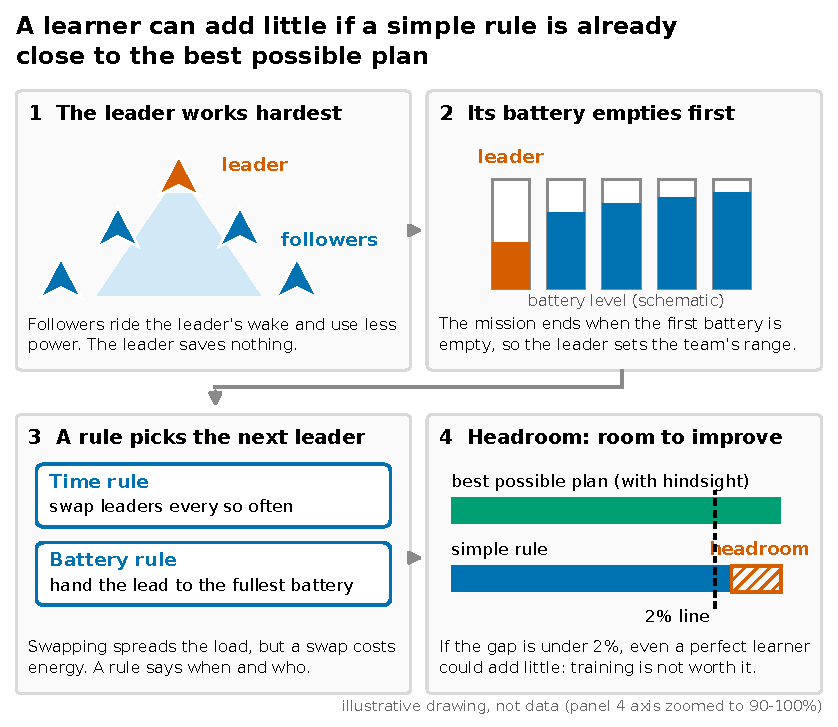
\includegraphics[width=0.64\textwidth]{figures/fig0_concept.pdf}
\caption{The headroom test asks how much room a rule leaves before any learning is tried. Panels 1 and 2 give the problem, panel 3 the kind of rule we test, and panel 4 the quantity we measure. Illustrative drawing, not data.}
\label{fig:concept}
\end{figure}

An \emph{upper bound} is the best score any policy could reach if it knew the future, computed offline for the same setting.
\emph{Headroom} is the relative gap between the two, and when the bound is valid it caps what any learned policy can add over the rule.
We study three problems: leader rotation, wake surfing (a follower holding the best spot behind the leader) and cooperative soaring (gliders sharing rising air); Table~\ref{tab:targets} lists what the rule is compared with in each.
Only leader rotation has an upper bound.
In the other two we compare the rule with a \emph{privileged reference}: a stronger controller given information that a deployable one would lack.

Reinforcement learning is a natural candidate for such allocation problems, but in the two soaring studies we read in full, the learned policy is not compared with a tuned hand-written rule \citep{reddy2016,flato2024}.
Training also needs a budget, tuning and several seeds in every setting, and a failed run cannot tell ``no room to improve'' from ``training went badly''.
So we ask first: how much better than a simple rule could any policy possibly be?
Its answer can be read whether or not a learner works.
We answer it with a \emph{headroom test}: predict first, then measure how far the best simple rule is from its comparison target.
A learner enters only after it passes a \emph{sanity gate}, which checks that a better-informed version of it can recover a gap known to exist.
The test came after an earlier experiment of ours (Appendix~\ref{app:history}).
In a 3-bird rotation game, a team trained with multi-agent PPO (MAPPO) \citep{yu2022mappo} only matched swapping leaders on a fixed timer, and it picked the highest-energy bird about as often as chance (Appendix~\ref{app:birds}).

We found three things.
In leader rotation, a rule that reads battery levels sits close to the bound in almost all settings.
One of our predictions said otherwise and missed by two orders of magnitude.
In wake surfing and soaring, stronger references do show gaps, but the conclusions we can draw from them are narrower.
When drones see only their neighbours, a gap remains, and our learner has not passed the check that would let us test it.

Three things we do not claim:
\begin{itemize}\setlength{\itemsep}{0pt}\setlength{\topsep}{0.2em}
\item We do not claim that learning has no value: a small gap says only that a learner cannot add much over the rule.
\item We do not claim that no setting leaves room for a learner: closeness to a reference is weaker evidence than closeness to an upper bound.
\item We make no priority claim: a limited web search (November 2026) found no study combining a written prediction, a rule-to-bound measurement and a sanity gate, though each idea has precedents (Section~\ref{sec:related}).
\end{itemize}

\section{Related Work}
\label{sec:related}

Drafting behind another aircraft saves energy in flight tests and models \citep{maskew1977,ray2002}.
Controllers that search for or hold the best wake position have been studied with extremum seeking \citep{binetti2003}, in simulation \citep{rossato2024} and in flight tests \citep{hanson2018}.

Reinforcement learning has been used to soar in simulated turbulence and in field flights \citep{reddy2016,reddy2018} and to fly cross-country on a real glider \citep{notter2023}.
One study reproduces vulture-like thermal soaring and states that it does not compare against rule-based controllers \citep{flato2024}.
We read the 2018 and 2023 papers only at abstract level and quote no numbers from them.

Against these groups, our contribution is not a new controller but a protocol.
It measures how far simple rules are from an upper bound before training, and it lets the learner in only after it passes a sanity gate.
Writing the prediction before the result borrows from preregistration \citep{nosek2018prereg}.
Bounds that let decisions use future information are called information relaxations in operations research \citep{brown2010information}; our hindsight bounds are of this kind.
Work on RL evaluation repeatedly warns that comparisons and statistics need care \citep{henderson2018matters,agarwal2021precipice}, and simple methods have matched deep RL on some benchmarks \citep{mania2018random,rajeswaran2017simplicity}.
Our learner is multi-agent PPO \citep{yu2022mappo}, which builds on PPO \citep{schulman2017ppo}.
We checked these method papers only at abstract level.
We found no citable precedent that treats the sanity gate as a formal requirement; it plays the role of a positive control in experimental science, and we first used such a gate in an earlier project of ours \citep{ho2026ladder}.

\section{The Headroom Test}
\label{sec:test}

We define headroom in a setting as $(U-R)/U$, where $R$ is the score of the best simple rule and $U$ the score of its comparison target.
We draw the line at 2\%, which we call the \emph{2\% line}: below it, we judge that training a learner is not worth trying.
The 2\% line is our own choice made before measuring, not a derived quantity, and a stricter line would change some conclusions (Section~\ref{sec:limits}).
Where the score is already a percentage, we report the gap in percentage points (pp).

The test has three steps.
First, we write down a prediction before measuring, for example ``about 30\% of settings will exceed 2\%''.
Second, we measure the rule and its comparison target in every setting of a grid.
Third, we compare the results with the prediction, including the predictions that failed.
The order, prediction first and results after, rests only on our own version-control timestamps, which anyone can set, so it is not third-party proof (Appendix~\ref{app:timeline}).
Table~\ref{tab:guess} sets our main guesses beside what happened. \IfFileExists{appendix_predictions.tex}{Appendix~\ref{app:scorecard} tallies all of them and, with Appendix~\ref{app:timeline}, notes which were written after earlier or partial results rather than blind.}{}

In \emph{leader rotation} each drone has a battery that drains fastest when the drone leads, and every swap of positions costs some energy.
The \emph{score} is how far the team flies before the first battery is empty.
A \emph{setting} is one combination of parameters, such as the number of drones, the swap cost, how much the drones differ and how noisy the drain is.
Two rules recur below: the \emph{time rule} hands the lead on at fixed intervals, and the \emph{battery rule} hands it to the drone with the most charge.
We study leader rotation at rising difficulty: a basic model, a richer model in which savings depend on position, and a noisy model in which the drain fluctuates (Appendix~\ref{app:model}).
A rule may see every drone's battery (a \emph{whole-team} rule) or only those of the drones next to it (a \emph{neighbours-only} rule).
In the example, a whole-team rule sees all three batteries, while a neighbours-only rule for drone C sees only B's.

\begin{table}[t]
\centering
\small
\caption{Each row compares the rule with a different kind of target, so read the last column before any result. Rotation rules are tuned per setting on the same instances, which favours them; wake and soaring controllers are tuned on separate seeds.}
\label{tab:targets}
\setlength{\tabcolsep}{4pt}
\begin{tabular}{@{}>{\raggedright\arraybackslash}p{2.6cm}>{\raggedright\arraybackslash}p{5.2cm}>{\raggedright\arraybackslash}p{7.4cm}@{}}
\toprule
Problem & What it asks & What the rule is compared with \\
\midrule
Leader rotation & Who should lead, and when should the lead change hands? & An offline upper bound that knows the future; it is computed by a solver, and some bounds are approximate or timed out (Appendix~\ref{app:evidence}) \\
Wake surfing & How closely can a controller keep a follower at the best spot behind the leader? & Privileged reference controllers (one knows the follower's true position, one has the same noisy GPS as the controller), which are not optima; the gap is in pp of total power \\
Cooperative soaring & How much room is left above a simple rule in which gliders announce the thermals they find? & The strongest method we tried, given the true thermal data; not a true optimum; the gap is in pp of the altitude ceiling \\
\bottomrule
\end{tabular}
\end{table}

A learner enters only through a sanity gate, a qualifying check.
Before running the real learner on any target setting, we train a better-informed version of it on control settings where an improvement over the neighbours-only rules is known to exist.
We call that improvement a \emph{known gap}.
We require it to recover at least half of that known gap, with a confidence interval above zero, in at least 2 of 3 control settings.
If it does not, its target-setting results are not interpreted.
The gate separates a failed learner from a setting without room, which a rule-versus-bound comparison alone cannot do.

\begin{figure}[tb]
\centering
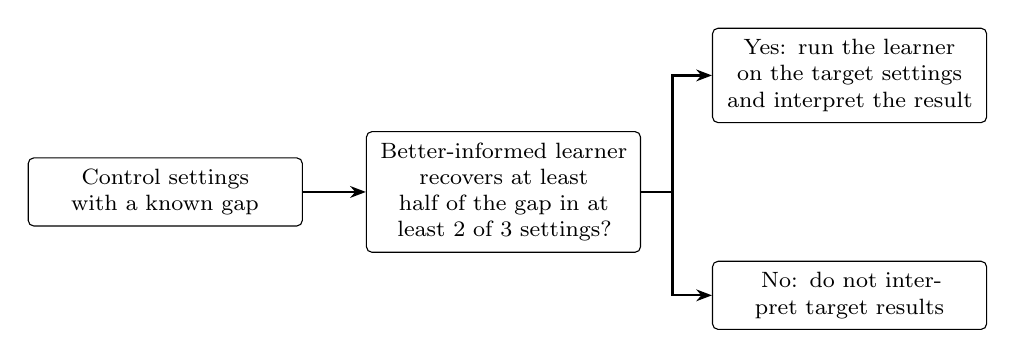
\begin{tikzpicture}[box/.style={draw,rounded corners=2pt,align=center,font=\footnotesize,inner sep=4pt,text width=3.2cm},arr/.style={-{Stealth[length=2mm]},thick}]
\node[box] (a) {Control settings with a known gap};
\node[box,right=8mm of a] (b) {Better-informed learner recovers at least half of the gap in at least 2 of 3 settings?};
\node[box,above right=1mm and 9mm of b] (y) {Yes: run the learner on the target settings and interpret the result};
\node[box,below right=1mm and 9mm of b] (n) {No: do not interpret target results};
\draw[arr] (a) -- (b);
\draw[arr] (b.east) -- ++(4mm,0) |- (y.west);
\draw[arr] (b.east) -- ++(4mm,0) |- (n.west);
\end{tikzpicture}
\caption{A learner is tested on the target settings only after it passes this qualifying check on control settings. Illustrative flow, not data.}
\label{fig:gatechart}
\end{figure}

\section{Results}
\label{sec:results}

We report the rule-to-target gap in 1120 leader-rotation settings, 108 wake-surfing settings and 11 soaring settings, with the quality of each comparison target stated.

\begin{table}[t]
\centering
\small
\caption{Our guesses were mixed, and the largest miss was expecting room where the drones differ most. The rows are a selection; Appendix~\ref{app:scorecard} tallies all of our predictions. Statements marked ``our reading'' or ``conjecture'' are untested.}
\label{tab:guess}
\begin{tabular}{@{}>{\raggedright\arraybackslash}p{0.25\textwidth}>{\raggedright\arraybackslash}p{0.32\textwidth}>{\raggedright\arraybackslash}p{0.36\textwidth}@{}}
\toprule
What we guessed & What happened & What we learned \\
\midrule
\textbf{Basic rotation.} A rule that reads battery levels stays within 2--3\% of the best plan when swapping is cheap.
& Right, and better: within 2\% in all but 4 of 192 settings, all at the highest swap cost.
& Measured: the time rule did far worse, more than 2\% from the best plan in 132 of 192 settings. \\
\addlinespace
\textbf{Richer rotation.} About 30\% of settings would leave more than 2\% of room, mostly where the drones differ most.
& Only 1 of 768 did, and none of the settings with large differences.
& Our reading, untested: when drones differ a lot, the best plan is simply to put the weakest drone where it saves most, which a rule does easily. \\
\addlinespace
\textbf{Wake surfing.} Gaps above 2 pp would appear only at large drift; with little or no drift they would stay below 2 pp.
& Half right. Little or no drift: at most 1.30 pp. Large random drift: also below 2 pp (at most 1.55). Gaps above 2 pp appeared only when the lead aircraft manoeuvred.
& Our reading, untested: at large drift even the references save at most 3.5 pp of power, so there is little to win. \\
\addlinespace
\textbf{Soaring.} Giving the simple rule the true thermal data would recover most of its gap to the strongest method.
& It did, and the strongest method's remaining lead was never confidently above 2 pp.
& Measured: the gap is mostly information, not decision structure. The reference is the best we tried, not an optimum. \\
\addlinespace
\textbf{Learner sanity gate.} The better-informed control learner would pass the sanity gate: 75\% chance on the first try, 35\% on the second.
& The first try passed in none of the three control settings; the second in one, where two were required.
& Measured: some runs still collapsed, so our diagnosis of the first failure, too little initial exploration, was at best incomplete. Our conjecture, untested: costly early swaps push the policy to swap too rarely. \\
\bottomrule
\end{tabular}
\end{table}

\subsection{A rule that reads battery levels sits close to the bound, contrary to our richer-model prediction}
\label{sec:close}
\label{sec:pred}

In the richer rotation model we predicted that about 30\% of settings would leave more than 2\% of headroom, and 1 of 768 did (Fig.~\ref{fig:pred}).
That one setting is a borderline case: its solver bound was not proven optimal (Appendix~\ref{app:evidence}).
The prediction pointed to settings with large drone differences, but none of those exceeds 2\%, so we moved to the next level instead of training there.

\begin{figure}[tb]
\centering
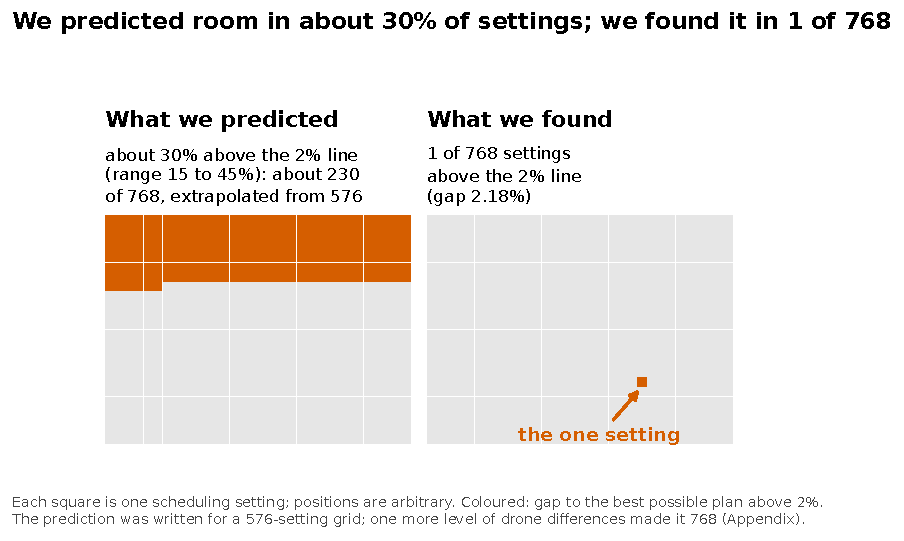
\includegraphics[width=0.55\textwidth]{figures/fig1_prediction.pdf}
\caption{We predicted that about 30\% of richer rotation settings would leave more than 2\% of headroom, and 1 of 768 did. The square positions are arbitrary.}
\label{fig:pred}
\end{figure}

A rule that reads battery levels is almost always within 2\% of the bound in leader rotation, while the time rule is often not (Fig.~\ref{fig:rot}).
In the basic model, 132 of 192 settings leave the time rule more than 2\% from the bound.
Across the basic and richer models, the battery rule alone is beyond the line in 8 of 960 settings (4 of 192 and 4 of 768; the 1 of 768 above takes the best of five rules).
In the noisy whole-team settings, all apparent excesses sit in the 62 of 160 settings whose bound timed out; such a bound is loose, which favours the learner side.

\begin{figure}[tb]
\centering
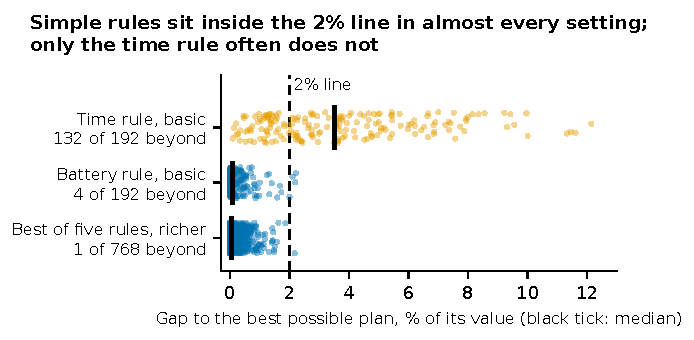
\includegraphics[width=0.55\textwidth]{figures/fig2a_rotation.pdf}
\caption{The battery rule sits close to the bound in almost every setting, while the time rule is often far above the 2\% line. Each dot is one setting; black tick: median; dashed line: the 2\% line. The bound is a solved fluid-model bound (Table~\ref{tab:evidence}).}
\label{fig:rot}
\end{figure}

\subsection{Wake surfing and soaring show gaps against stronger references, but support narrower conclusions}
\label{sec:wakesoar}

For wake surfing, the answer depends on which privileged reference we compare against (Appendix Fig.~\ref{fig:wake}).
One reference, the one in our prediction, knows the follower's true position.
Against it, 16 of 108 settings are beyond the line, all of them when the lead aircraft manoeuvres.
These 16 come from 4 of 27 distinct conditions (Appendix~\ref{app:wake}).
A second reference, given the same noisy GPS as the controller, shows at most 1.77 pp, but the classical controller sometimes beats it, so it is a diagnostic, not a cap on a learner.

For soaring, the large differences we found come from information rather than decision structure (Appendix Fig.~\ref{fig:soar}).
The simple rule has each glider announce the thermals it finds.
The strongest method we tried also gets the true parameters of detected thermals (information) and plans its moves differently (decision structure).
It beats the simple rule by more than 2 pp with confidence in 10 of all 11 settings.
Against the simple rule's decision structure given the same data, its lead is never confidently above 2 pp (Appendix~\ref{app:evidence}).
With only observed estimates, even the strongest decision structure does worse than the simple rule in all 11 settings.
Here the reference is ``the best we tried'' rather than a true optimum, so a better planner or a learned policy could do more.
Our result only says that, given the same data, we found no sign of room in decision structure.

\subsection{When drones see only their neighbours, a gap remains, and our learner has not passed the check needed to test it}
\label{sec:l3}
\label{sec:gate}

The clearest remaining gap appears when each drone sees only its neighbours and the drain is noisy and correlated, and we leave it unresolved (Fig.~\ref{fig:l3}).
We examine 23 of the 160 noisy settings; they were selected because they showed a gap, so they overstate how common it is.
In them, the best neighbours-only rule trails the whole-team rule by a median 1.41\% of the bound.

\begin{figure}[tb]
\centering
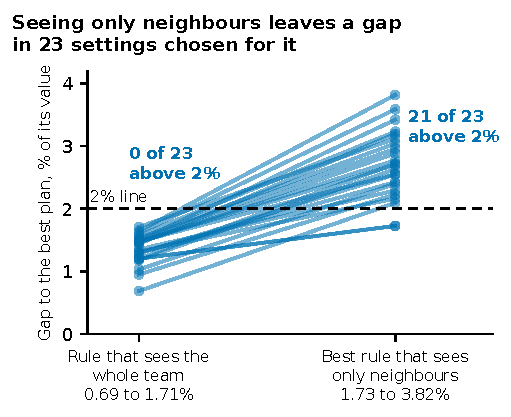
\includegraphics[width=0.46\textwidth]{figures/fig3_local_gap.pdf}
\caption{In 21 of the 23 settings the neighbours-only rule is more than 2\% from the bound, against none for the whole-team rule. Each line is one of 23 settings selected because the time rule exceeded 2\%, so they overstate how common the gap is; 20 are 5-drone, correlated-noise, identical-drone settings. The neighbours-only rule falls short of the whole-team rule by a median 1.41\% of the bound (0.52 to 2.17).}
\label{fig:l3}
\end{figure}

To ask whether learning can close this gap, a learner first has to pass the sanity gate.
The control version is given whole-team information and a ready-made swap action, so a pass would show only that the training set-up works.
The first preregistered attempt passed in none of the three control settings; a second, which changed the learner's initial exploration and used more seeds, passed in one, where two were required (Fig.~\ref{fig:gate}; Appendix~\ref{app:gate}).
The second attempt also met a refutation condition we had written down beforehand: our diagnosis of the first failure, too little initial exploration, was at best incomplete.
Following the preregistration, we did not make the real run on the 23 target settings and did not write a third attempt.
Without the gate, a poor result from the neighbours-only learner could have been read as evidence that no learner can close the gap.
With it, the correct reading is that this learner setting cannot yet recover a gap that a rule is known to recover, so it says nothing about the neighbours-only settings.

\begin{figure}[tb]
\centering
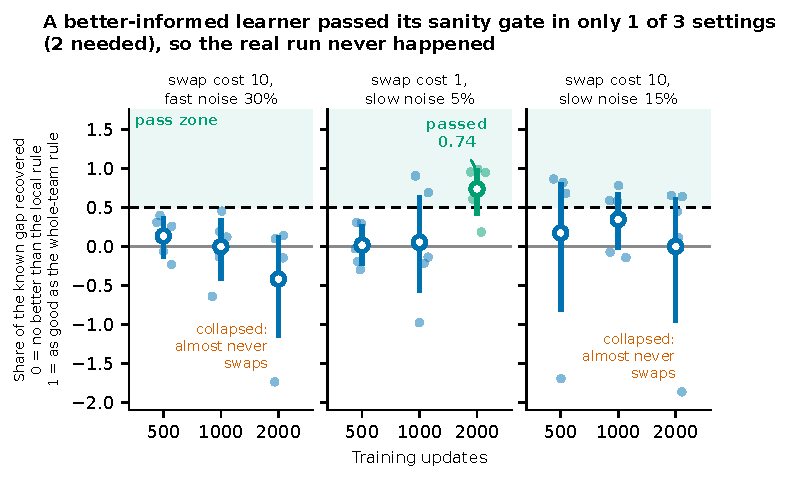
\includegraphics[width=0.6\textwidth]{figures/fig4_sanity_gate.pdf}
\caption{The better-informed control learner passes the sanity gate in 1 of 3 control settings, where 2 were required. Sanity gate of the second preregistration, run with whole-team features. Dots: 5 seeds; ring and bar: mean and 95\% interval; dashed line: pass line. Only the middle panel at 2000 updates passes.}
\label{fig:gate}
\end{figure}

\section{Limitations}
\label{sec:limits}

Five limits matter most; Appendix~\ref{app:limits} gives the full list.
\begin{itemize}\setlength{\itemsep}{0pt}\setlength{\topsep}{0.2em}
\item Two biases pull in opposite directions. Rotation rules are tuned on the same instances that score them and, in the richer model, the best of five is chosen after the fact; both favour the rules. Solver bounds that timed out are loose, which favours the learner side. We did not quantify the net effect.
\item The 2\% line is our own choice, and a stricter 1\% line would change some conclusions, wake surfing most.
\item All results come from simulation with assumed physics, and the model gives followers larger savings than flight tests show (Appendix~\ref{app:formation}).
\item The test is necessary rather than sufficient: a small gap says a learner cannot add much over the rule, not that learning has no other value, such as avoiding hand design.
\item Our MAPPO study covers one policy class, one reward and one set of hyperparameters per preregistration.
\end{itemize}

\section{Conclusion}

A check made before training showed that a simple rule that reads battery levels sits close to the upper bound in the basic and richer leader-rotation models: within 2\% in all but 8 of 960 settings.
The process corrected us twice: measuring first kept us from training where the prediction pointed, and the sanity gate kept a failed training run from being read as evidence about learning.
In soaring and wake surfing the reference is not a cap: we have not shown that a learner has room there, and we have not shown that it has none.
The neighbours-only gap in leader rotation is real in the 23 settings we examined and remains unresolved.
Our learner did not pass its own sanity gate, so whether learning can close that gap remains an open question.

\section*{Author contributions}
The author set the research question, made every change of direction and proposed the direction of each prediction; AI coding agents expanded these into the written prediction files. Most of the code, the running of the experiments, the analysis and the drafting of this paper were carried out by AI coding agents (Anthropic's Claude models, used through Claude Code) working under the author's direction; internal reviews of the drafts were also simulated with AI agents. The author takes full responsibility for the content. This is separate from the language-model commander of Appendix~\ref{app:llm}, an object of study.

\bibliographystyle{plainnat}
\bibliography{refs}

\clearpage
\appendix

\section{Full evidence by family}
\label{app:evidence}

This appendix gives the numbers behind Section~\ref{sec:results}, family by family.

\begin{table}[t]
\centering
\footnotesize
\caption{Evidence by family. The unit differs by row and the quality of the bound differs too, so read the last column before the result column. ``Beyond'' means above the 2-unit line. Rotation rules are tuned per setting on the same instances, which favours them; wake and soaring controllers are tuned on separate seeds.}
\label{tab:evidence}
\setlength{\tabcolsep}{3.5pt}
\begin{tabular}{@{}>{\raggedright\arraybackslash}p{2.0cm}>{\raggedright\arraybackslash}p{1.2cm}>{\raggedright\arraybackslash}p{1.4cm}>{\raggedright\arraybackslash}p{5.5cm}>{\raggedright\arraybackslash}p{5.2cm}@{}}
\toprule
Family & Settings & Unit & Result & What the bound is \\
\midrule
Rotation, basic & 192 & \% of bound & Battery rule: 4 beyond, max 2.22. Time rule: 132 beyond, max 12.14 & Solved fluid-model bound, not the discrete optimum (off by about 0.1\%) \\
Rotation, richer (position-aware) & 768 & \% of bound & Battery rule: 4 beyond, max 2.33. Best of 5 rules: 1 beyond (2.18), median 0.045 & Same kind of bound, looser at high swap cost; in 152 settings the solver did not prove optimality and a dual bound overstates the gap \\
Rotation, noisy, whole-team information & 160 & \% of bound & 98 settings with a trusted bound: max 1.71. In 62 settings the bound timed out, and over a third of those look beyond the line & Hindsight bound that knows all noise, loose, timed out in 62 settings; 20-step time blocks make it not strictly guaranteed (block check within 0.15\%) \\
Rotation, noisy, neighbours only & 23 of the 160 & \% of bound & Neighbours-only rule 1.73 to 3.82; whole-team rule 0.69 to 1.71 & Same as above; settings selected for a gap \\
Wake surfing & 108 & pp of total power & Perfect-position reference (in our prediction): 16 beyond, max 2.79. Same-noisy-GPS reference (diagnostic): max 1.77 (95\% CI up to 1.83), none beyond & Privileged controllers, not optima; the classical controller beats the same-GPS one in 34 of 108 settings (worst $-0.24$) \\
Cooperative soaring & 11 (8 with 5 gliders) & pp of altitude ceiling & Strongest method vs simple rule: above 2 with confidence in 10 of 11 (5.9 to 13.9 in 4 informative 5-glider settings). Vs simple decisions given the same true data: max $+2.5$ [0.1, 5.1], none with interval above 2 & Strongest method we tried, given true thermal data; not a true optimum \\
\bottomrule
\end{tabular}
\end{table}

\subsection{Leader rotation}

In the richer rotation model we predicted that about 30\% of settings would leave more than 2\% of headroom, and 1 of 768 did (Fig.~\ref{fig:pred}).
That setting shows a gap of 2.18\%, and its solver bound was not proven optimal; against the best solution found the gap is 1.89\%.
The wake-surfing prediction missed too: we expected a largest gap of 3 to 5 pp, and the largest was 2.79 pp against the perfect-position reference and 1.77 pp against the same-GPS reference.
Our plan, fixed before this level, was to train a learner only where a gap appeared. The prediction pointed to settings with large drone differences, but none of those exceeds 2\% (largest 0.59\%), so we moved to the next level instead of training there.

A rule that reads battery levels is almost always within 2\% of the bound in leader rotation, while the time rule is often not (Fig.~\ref{fig:rot}).
In the basic model, 132 of 192 settings leave the time rule more than 2\% from the bound (maximum 12.14\%).
The battery rule is beyond the line in only 4 of those settings (maximum 2.22\%, median 0.095\%).
In the richer model the battery rule alone is beyond the line in 4 of 768 settings (maximum 2.33\%), and the best of five rules in 1, with a median gap of 0.045\%.
In the noisy settings with whole-team information, the maximum is 1.71\% where the bound is trusted, and all apparent excesses sit in the 62 settings whose bound timed out (Table~\ref{tab:evidence}).

\subsection{Wake surfing}

For wake surfing, the answer depends on which privileged reference we compare against (Fig.~\ref{fig:wake}).
The best classical controller, in most settings, filters its sensors to estimate where the wake is.
Against a reference that also knows its own position perfectly, as in our prediction, 16 settings are beyond the line: all 12 where the lead aircraft weaves and 4 of 12 where it steps.
The largest gap there is 2.79 pp.
A reference given the same noisy GPS as the controller stays within 1.77 pp (95\% interval at most 1.83 pp), but it is a diagnostic, not a cap on a learner. Like a learner, it has no perfect position, but it was not in our prediction. The classical controller beats it in 34 of 108 settings (22 with the 95\% interval below zero, worst 0.24 pp) because it also reads roll moment, which the reference does not and a learner could.

The 16 settings beyond 2 pp are point estimates; in 14 of them the lower end of the 95\% interval also exceeds 2 pp.

\begin{figure}[tb]
\centering
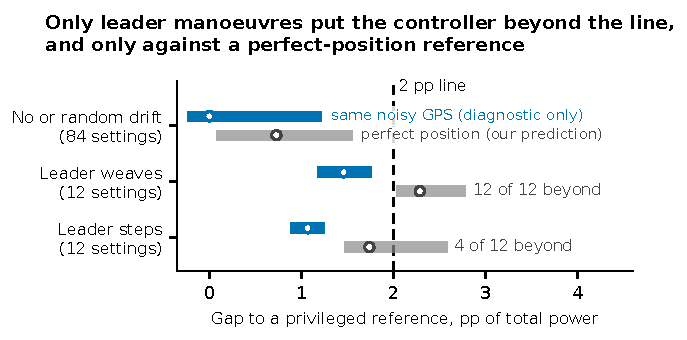
\includegraphics[width=0.66\textwidth]{figures/fig2b_wake.pdf}
\caption{The answer depends on the reference: against the perfect-position reference some settings are beyond 2 pp, against the same-GPS reference none are. Bar: range over the settings in a row; ring: median; dashed line: 2~pp. The bound is a privileged reference, not an optimum (Table~\ref{tab:evidence}).}
\label{fig:wake}
\end{figure}

\subsection{Cooperative soaring}

For soaring, the large differences we found come from information rather than decision structure (Fig.~\ref{fig:soar}).
Announcing found thermals gains 5.6 to 24.2 pp of altitude over flying alone in the four long-lived-thermal settings with five gliders.
These four long-lived-thermal settings are not the same four as the informative settings of Fig.~\ref{fig:soar}: the former include a setting where most simple-rule gliders land and leave out one the latter include.
The strongest method we tried, which is given the true parameters of detected thermals, beats the simple rule by 5.9 to 13.9 pp in the four informative 5-glider settings, and by more than 2 pp with confidence in 10 of all 11. Against the simple rule's decision structure given the same data, its lead is at most $+2.5$ pp [0.1, 5.1], and no interval lies above 2 pp.
With only observed estimates, even the strongest decision structure does worse than the simple rule in all 11 settings (by 0.2 to 24.5 pp).
Here the bound is ``the best we tried'' rather than a true optimum, so a better planner or a learned policy could do more; our result only says that, given the same data, we found no sign of room in decision structure.

\begin{figure}[tb]
\centering
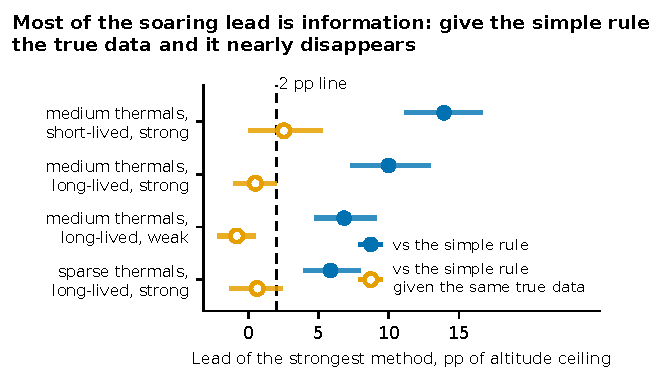
\includegraphics[width=0.66\textwidth]{figures/fig2c_soaring.pdf}
\caption{Once the simple rule is given the same data, the strongest method's lead is no longer confidently above 2~pp in any setting. Four informative 5-glider settings (the other four, where most simple-rule gliders land, are left out). Dot: estimate; bar: 95\% interval. Across all 11 settings the lead over the simple rule is confidently above 2~pp in 10, and over the simple rule given the same data in none. The bound is the strongest method we tried.}
\label{fig:soar}
\end{figure}

\subsection{Neighbours-only gap}

The clearest remaining gap appears when each drone sees only its neighbours and the drain is noisy and correlated, and we leave it unresolved (Fig.~\ref{fig:l3}).
Of the 98 noisy settings with a trusted bound, 23 are settings where the time rule is more than 2\% from the bound.
In those 23, the best neighbours-only rule is 1.73 to 3.82\% from the bound, and the whole-team rule is 0.69 to 1.71\%.
Here the neighbours-only rule is the better of the time rule and a neighbour-swap rule.
It trails the whole-team rule by 0.52 to 2.17\% of the bound (median 1.41\%), and 21 of the 23 neighbours-only gaps exceed 2\% against none of the whole-team gaps.

\section{Leader-rotation model and settings}
\label{app:model}

\emph{Leader rotation} is an energy-bucket model in which each of $N$ drones carries a battery treated as a bucket that drains at a rate set by its position in the formation: the leader drains at the full rate and followers at a reduced rate that depends on position, since the wake effect is stronger further back.
A swap of two positions costs energy ($c$ units), and the mission ends when the first bucket is empty, so the score is the team's normalized flight range.
The basic level has two position classes and a grid of 192 settings.
The richer level uses position-dependent savings and 768 settings, spanning $N \in \{3,5,7,10\}$, V and echelon layouts, two position sets, an induced-drag share $f_{ind} \in \{0.3, 0.4, 0.5\}$, swap costs $c \in \{0,1,3,10\}$ and drone-difference levels $h \in \{0, \pm 5\%, \pm 15\%, \pm 30\%\}$ of the drain rate; the prediction was written for 576 of these settings, before the $\pm 5\%$ level was added.
The noisy level adds per-step drain noise (independent or AR(1) with correlation length 10 or 50 steps, standard deviation 5, 15 or 30\%) and, with probability 0.2, a permanent 20\% drain increase of one drone in mid-mission; it has 160 settings (16 without per-step noise) with $N \in \{5,10\}$, $c \in \{1,10\}$, $f_{ind}=0.4$ and $h \in \{0, \pm 15\%\}$.
Rules are evaluated on 200 instances per setting, except where nothing is random (the richer-level settings with $h=0$ and the noisy-level settings with no noise, no event and $h=0$), which are deterministic and use a single instance; the hindsight bound uses the first 60 of the instances in the noisy level.
The richer level's five rules are fixed positions, a time rule, a battery rule that swaps the lead with the drone of most remaining range once the difference exceeds a margin, a periodic sort by remaining range, and a single swap made only when its predicted gain exceeds its cost. The noisy level keeps the first three and adds a battery rule that also estimates each drone's own drain and a neighbours-only rule that swaps two adjacent positions when the drone in the costlier position has at least a margin less remaining range than its neighbour.
We evaluate the neighbours-only chain with adjacent-position swaps, and we did not test other local protocols.
The solver's time limit is 5 seconds of wall-clock time per solve (60 seconds in the block-size check), and four worker processes ran in parallel, so the number of settings that time out may differ on another machine.

\section{Wake-surfing details}
\label{app:wake}

A follower holds a lateral and vertical offset behind a leader, and the saving depends on the offset; we test controllers under drift of the vortex position, GPS noise (correlated, 0.02 to 0.08 wingspans), power-measurement noise and roll-moment noise, 12 settings per drift scenario and 64 evaluation seeds per setting.
The controllers are a fixed set point, an extended-Kalman-filter set point, and extremum seeking, each tuned on separate seeds.
Table~\ref{tab:wake} lists both privileged references.

\begin{table}[h]
\centering
\small
\caption{Wake surfing: gap (min / median / max, pp of total power) of the best classical controller to the two privileged references, per drift scenario (12 settings each).}
\label{tab:wake}
\begin{tabular}{@{}lccc@{}}
\toprule
Scenario & Same-GPS reference & Perfect-position reference & Beyond 2 pp \\
\midrule
No drift & $-0.24$ / $-0.06$ / $-0.01$ & 0.25 / 0.76 / 1.30 & 0 \\
Small, fast & $-0.09$ / $-0.03$ / $-0.02$ & 0.13 / 0.47 / 1.01 & 0 \\
Small, slow & $-0.01$ / 0.04 / 0.12 & 0.36 / 0.73 / 1.29 & 0 \\
Medium, fast & $-0.01$ / 0.00 / 0.00 & 0.14 / 0.32 / 0.59 & 0 \\
Medium, slow & 0.50 / 0.58 / 0.92 & 0.89 / 1.14 / 1.41 & 0 \\
Large, fast & 0.00 / 0.00 / 0.00 & 0.07 / 0.14 / 0.29 & 0 \\
Large, slow & 0.82 / 1.06 / 1.21 & 0.88 / 1.20 / 1.55 & 0 \\
Leader weaves & 1.18 / 1.46 / 1.77 & 2.04 / 2.29 / 2.79 & 12 \\
Leader steps & 0.89 / 1.07 / 1.25 & 1.47 / 1.74 / 2.58 & 4 \\
\bottomrule
\end{tabular}
\end{table}

The weave and step manoeuvres use amplitudes and a period that we chose, and the weave result is sensitive to its period, which we did not scan.
The 108 settings are 27 conditions (a drift scenario crossed with a GPS noise level), each paired with 4 sensing-noise combinations, and the settings within a condition share one simulation of the reference.
The 16 settings beyond 2 pp all lie in 4 of the 27 conditions, each a complete group of four settings; the 52 settings beyond 1 pp lie in 15 of the 27 conditions.

\section{Cooperative-soaring details}
\label{app:soaring}

Gliders start at 1600 m under a 3200 m ceiling, sink at 1 m/s, fly at 12 m/s for 2400 s, and look for thermals with density (sparse or medium), lifetime (short or long) and strength (updraft equal to 1.5 or 3 times the sink rate) varied over 8 settings with 5 gliders, plus 3 settings with 10.
The ladder is: no sharing, announcing found thermals (the simple rule), two intermediate designs, and the strongest method, which is given the true position and strength of thermals already detected.
One intermediate design keeps the simple rule's decision structure but uses true thermal data; the other keeps the strongest method's decision structure but uses only observed estimates.
The metric is the time-averaged altitude of the lowest glider as a percentage of the ceiling, with 60 evaluation seeds per setting and paired bootstrap intervals.
A setting is ``uninformative'' when at least half of the simple-rule gliders land; 4 of the 8 five-glider settings are in that group, and we leave them out of Fig.~\ref{fig:soar}.
An earlier information-matched planner lost to the simple rule and was recorded as undecided, not as evidence of no room. Round 1 used a lower start and ceiling and scored time airborne; after its floor effects we doubled the heights and changed the score, so its prediction does not bear on these numbers.

\section{Sanity-gate runs in detail}
\label{app:gate}

This appendix gives the full account of the sanity-gate runs summarised in Section~\ref{sec:gate}.

We first trained a MAPPO learner with whole-team features on three of the 23 settings, before any real run of the neighbours-only learner, and it did not pass the gate.
The control version of the learner is given whole-team features and a ``swap with the drone of most remaining range'' action, so a pass would show only that its optimizer, reward and network are adequate.
In the first preregistration no control setting passed at 500, 1000 or 2000 training updates (0 of 3 each time; the best mean was 0.29).
We then wrote a second preregistration that changed only the learner's initial exploration, lowering the starting bias toward ``do nothing'' from $+5$ to $+2$, and used 5 seeds instead of 3.
That version passed 0 of 3 settings at 500 and 1000 updates and 1 of 3 at 2000 (Fig.~\ref{fig:gate}).
The passing setting recovered 0.74 of the gap (95\% CI 0.43 to 0.97), against a pass line of 0.5 with 2 passing settings required.

The second run also met our own refutation condition for the diagnosis.
At 2000 updates, 2 of 15 runs still collapsed to almost never swapping (recovered-gap shares of $-1.74$ and $-1.87$; policy entropy 0.004), so the explanation that low initial entropy caused the collapses was at best incomplete.
Both collapses were in high swap-cost settings, and we conjecture, without testing, that early swaps are punished by their cost so that the policy learns to swap too rarely.
Following the preregistration, we did not make the real run on the 23 target settings and did not write a third attempt.
Without the gate, a poor result from the neighbours-only learner could have been read as ``learning cannot close the gap''; the gate showed first that even the better-informed version scored between $-2.5$ and $+0.3$ in the first preregistration.
With it, the correct reading is that this learner setting cannot yet recover a gap that is known to be recoverable by a rule, so it says nothing about the neighbours-only settings.

\section{Preregistration details for the neighbours-only learner}
\label{app:mappo}

Each preregistration fixed the gate rule in advance: if the control version does not pass, the target-setting results are not interpreted, and the hyperparameters may not be changed after the fact; any change requires a new written preregistration.

\begin{table}[ht]
\centering
\footnotesize
\caption{Share of the known gap recovered (mean, 95\% CI) in the three control settings (swap cost, noise correlation, noise size). First preregistration: 3 seeds, initial ``do nothing'' bias $+5$. Second: 5 seeds, bias $+2$.}
\label{tab:mappo}
\begin{tabular}{@{}llccc@{}}
\toprule
Version & Updates & cost 10, fast 30\% & cost 1, slow 5\% & cost 10, slow 15\% \\
\midrule
v1 & 500 & $-1.15$ [$-2.02$, $-0.02$] & $-2.52$ [$-4.57$, 0.43] & $-0.30$ [$-1.89$, 0.60] \\
v1 & 1000 & $-0.44$ [$-1.77$, 0.43] & $-0.61$ [$-2.24$, 0.51] & $-0.26$ [$-1.81$, 0.63] \\
v1 & 2000 & $-0.34$ [$-1.69$, 0.47] & 0.29 [$-0.30$, 0.78] & $-0.32$ [$-1.81$, 0.55] \\
v2 & 500 & 0.13 [$-0.13$, 0.35] & 0.01 [$-0.22$, 0.25] & 0.17 [$-0.80$, 0.79] \\
v2 & 1000 & $-0.00$ [$-0.41$, 0.33] & 0.05 [$-0.57$, 0.62] & 0.34 [$-0.01$, 0.66] \\
v2 & 2000 & $-0.42$ [$-1.14$, 0.10] & \textbf{0.74} [0.43, 0.97] & $-0.00$ [$-0.95$, 0.60] \\
\bottomrule
\end{tabular}
\end{table}

The learner uses two-layer 64-unit tanh networks for actor and critic, decisions every 5 simulation steps, a team reward equal to the range gained, 256 episodes per update, and evaluation on the same 200 instances as the rules; the control version adds whole-team features and a swap-with-most-remaining-range action.
The first preregistration gave a 75\% chance of passing by 2000 updates, and it did not pass. The second gave 35\%, so its failure was within what we expected, although its predicted median recovery at 2000 updates (0.35) was above the observed $-0.00$.
The target run was never executed; the only neighbours-only runs were wiring tests of at most 20 updates on one of the 23 settings, before the first preregistration.
Reproduction commands are in the repository (\texttt{scripts/l3\_mappo\_vmap.py}, \texttt{scripts/l3\_analyze.py}).

\section{All limitations}
\label{app:limits}

This appendix gives the full list of limitations; Section~\ref{sec:limits} keeps the five that matter most.

All results come from simulation with assumed physics: the share of induced drag in total power is assumed and swept from 0.3 to 0.5, not measured, and the model gives followers larger savings than flight tests show (Appendix~\ref{app:formation}).
The 2\% line is our choice; with a 1\% line, 11 of 192 basic-rotation settings (battery rule), 22 of 768 richer-rotation settings (best of five rules) and 52 of 108 wake-surfing settings (perfect-position reference; 28 against the same-GPS one) would be beyond it.
Rotation rules are tuned per setting on the same instances used for scoring and, in the richer model, chosen after the fact among five, which favours them; the solver bounds that timed out favour the learner side, and we did not quantify the net effect.
The three bounds differ in kind (Table~\ref{tab:evidence}), and for soaring and for wake surfing a reference is not an optimum, so ``close to the bound'' is weaker evidence there than in rotation.
The test is necessary rather than sufficient: a small gap says a learner cannot add much over the rule, not that learning has no other value, such as avoiding hand design.
No setting is known to have headroom for a learned policy in particular, which is why the sanity gate matters and why our failure to pass it limits what we can say about the neighbours-only settings.
Timestamps come from git and can be set by the author, and our MAPPO study covers one policy class, one reward and one set of hyperparameters per preregistration.
Two further lines, a 3-bird game and a language-model commander, are small and in the appendix (Appendices~\ref{app:birds} and~\ref{app:llm}).
The intervals we report reflect only the variation across evaluation seeds, not the variation from tuning.

\section{Cost and history}
\label{app:history}

This appendix holds the cost figures and the research history that the introduction leaves out.

Measuring a rule against a bound is not free either: the 928 richer and noisy rotation settings took about 10 CPU-hours (38 CPU-seconds each), against about 200 GPU-seconds per setting to train 5 seeds.
CPU seconds and GPU seconds cannot be compared directly, and the GPU figure does not include tuning.
An earlier RL experiment of ours, a 3-bird rotation game trained with multi-agent PPO (MAPPO), matched a fixed-time rotation (normalized score difference $+0.013 \pm 0.017$, 3 seeds; the $\pm$ values are 95\% $t$ intervals over 3 seeds) without learning to choose leaders by energy (Appendix~\ref{app:birds}).
The idea of measuring first came later, from a review of our drone plan that warned a simple rule might leave a learner nothing to learn.

\section{Prediction and result timeline}
\label{app:timeline}

\begin{table}[h]
\centering
\small
\caption{Git author times of the prediction and the result commit for each family (UTC+8). Times can be set by the author, and the two learner gaps include GPU queueing and a pause. The commit hashes belong to the author's private development repository. The public repository is a clean export without that history, and its file \texttt{docs/provenance.md} lists each of these commits with its hash, author time and title. The order of events in this table is therefore the author's statement, and there is no third-party timestamp behind it. The prediction files in \texttt{docs/predictions/} of the public repository are copies in which a few passages are masked (internal role wording about the author, and local resource settings); each masked place is marked, and the git blob identifiers of the unmasked originals are listed in \texttt{docs/provenance.md}.}
\label{tab:timeline}
\begin{tabular}{@{}lllr@{}}
\toprule
Family & Prediction & Result & Gap \\
\midrule
Birds v2 & 10-31 14:21 (2838e68) & 10-31 19:56 (98937d9) & 5 h 35 min \\
Rotation, basic & 10-31 22:38 (a0619ab) & 10-31 23:09 (a7e76aa) & 31 min \\
Rotation, richer & 11-01 11:15 (79b4dbc) & 11-01 13:26 (3c774e7) & 2 h 11 min \\
Rotation, noisy & 11-01 13:28 (e8d6059) & 11-01 15:00 (ae62fc8) & 1 h 32 min \\
Wake surfing & 11-01 19:59 (f49e6e8) & 11-01 20:05 (3437930) & 6 min \\
Soaring, round 1 & 11-01 20:24 (071574f) & 11-01 22:48 (a477e3b) & 2 h 24 min \\
Soaring, round 2 & 11-01 22:58 (4eacb94) & 11-01 23:27 (3219473) & 29 min \\
Soaring, round 3 & 11-02 10:44 (02dc53f) & 11-02 11:04 (7c215c2) & 20 min \\
Language-model commander & 11-02 23:29 (5c53a88) & 11-02 23:32 (f1c439d) & 3 min \\
Neighbours-only learner, first & 11-04 21:33 (38ce89e) & 11-06 00:18 (74245e9) & 26 h 45 min \\
Neighbours-only learner, second & 11-06 00:22 (0e16639) & 11-06 14:06 (040f391) & 13 h 44 min \\
\bottomrule
\end{tabular}
\end{table}

Three disclosures apply to this timeline.
The prediction for soaring round 2 was written after two small trial runs, and its writer had seen rough numbers from them.
The prediction for soaring round 3 was written after we had seen the round-2 results.
The version-control commits that hold the predictions do not freeze the code and the grid at the same time.

\IfFileExists{appendix_predictions.tex}{% Auto-generated by scripts/gen_scorecard.py (rows in scripts/scorecard_rows.py); do not edit by hand.
\section{All predictions and how they fared}\label{app:scorecard}

This table summarises how the predictions written for this project fared. Verdicts are those we recorded at the time or, where our records give numbers but no verdict, those we assigned when compiling this table. A prediction stated as a probability is scored by its more likely side. The row-by-row table is in the supplement (\path{supplement_predictions.pdf}) and in \path{docs/predictions/scorecard_sources.md}.

\begin{center}\small
\begin{tabular}{@{}l>{\raggedleft\arraybackslash}p{0.8in}>{\raggedleft\arraybackslash}p{0.38in}>{\raggedleft\arraybackslash}p{0.5in}>{\raggedleft\arraybackslash}p{0.45in}>{\raggedleft\arraybackslash}p{0.62in}>{\raggedleft\arraybackslash}p{0.75in}@{}}
\toprule
Family & Predictions & Held & Held partly & Failed & Not assessed & Verdicts assigned for this table \\
\midrule
Birds v2 & 5 & 4 & 0 & 1 & 0 & 0 \\
Rotation basic & 12 & 5 & 3 & 4 & 0 & 2 \\
Rotation richer & 14 & 4 & 4 & 5 & 1 & 1 \\
Rotation noisy & 11 & 3 & 5 & 3 & 0 & 1 \\
Wake surfing & 12 & 5 & 1 & 5 & 1 & 2 \\
Soaring round 1 & 18 & 6 & 4 & 4 & 4 & 2 \\
Soaring round 2 & 14 & 5 & 7 & 2 & 0 & 8 \\
Soaring round 3 & 9 & 6 & 2 & 1 & 0 & 6 \\
Language-model commander & 12 & 6 & 1 & 5 & 0 & 10 \\
Neighbours-only learner first & 2 & 0 & 0 & 1 & 1 & 0 \\
Neighbours-only learner second & 4 & 1 & 0 & 3 & 0 & 2 \\
\midrule
Total & 113 & 45 & 27 & 34 & 7 & 34 \\
\bottomrule
\end{tabular}
\end{center}

Some of our predictions were written after earlier results or small trial runs: soaring round 2 after two trial runs (\path{soaring_headroom2/PREDICTION.md}, line 3), round 3 after the round-2 results (\path{soaring_headroom3/PREDICTION.md}, line 3), noisy rotation after the richer-rotation results (\path{drone_bucket/PREDICTION_L23.md}, line 3), the language-model commander after a look at the oracle (\path{llm_commander/PREDICTION.md}, line 5), and the second learner after the first one failed (\path{l3_mappo_prereg_v2.md}, section 0). The richer-rotation prediction covered 576 settings, but 768 were measured because we added a $\pm$5\% level (\path{drone_bucket/PREDICTION_L1.md}, line 4; \path{drone_bucket_l1.md}, line 22). Verdicts such as ``too high'', ``too low'' or ``right direction, wrong size'' were all recorded as held partly; we chose this mapping when compiling this table (\path{scorecard_sources.md}, section 1).
}{}

\section{A 3-bird rotation game}
\label{app:birds}

A 3-agent survival game with a team reward (MAPPO, energy-aware observation, 3 seeds, $5\times 10^7$ steps, 512 evaluation episodes) reached a normalized reward of $1.001 \pm 0.017$, which is $+0.013 \pm 0.017$ above a fixed-time rotation (0.9875); a simple energy-gate rule reached 1.0284.
The $\pm$ values are 95\% $t$ intervals over 3 seeds.
The policy handed the lead to the highest-energy bird 34\% of the time, about the chance rate of 33\%.
Independent-learner and individual-reward variants mostly collapsed to a fixed leader.
Observational evidence also found no support for energy-driven rotation in real birds \citep{voelkl2015}.

\section{A language-model commander}
\label{app:llm}

Two models, referred to only by the aliases ``Haiku'' and ``Sonnet'' (called on 2026-11-02; exact version strings were not recorded), each translated 14 natural-language instructions into rule parameters for the richer rotation model.
Both gave valid answers that obeyed the hard constraints in 14 of 14 instructions, and the largest regret against an exhaustive search under the same constraints was 1.15\% and 1.31\%.
The test was too lenient to separate the two models, and we had predicted otherwise (compliance of 71\% and 86\%), so the prediction failed.
Each model answered once, all 14 instructions in one call, and each call included one tool use whose content we did not inspect.
This line is a small demonstration, not support for the headroom claim.

\section{Formation physics}
\label{app:formation}

\begin{figure}[h]
\centering
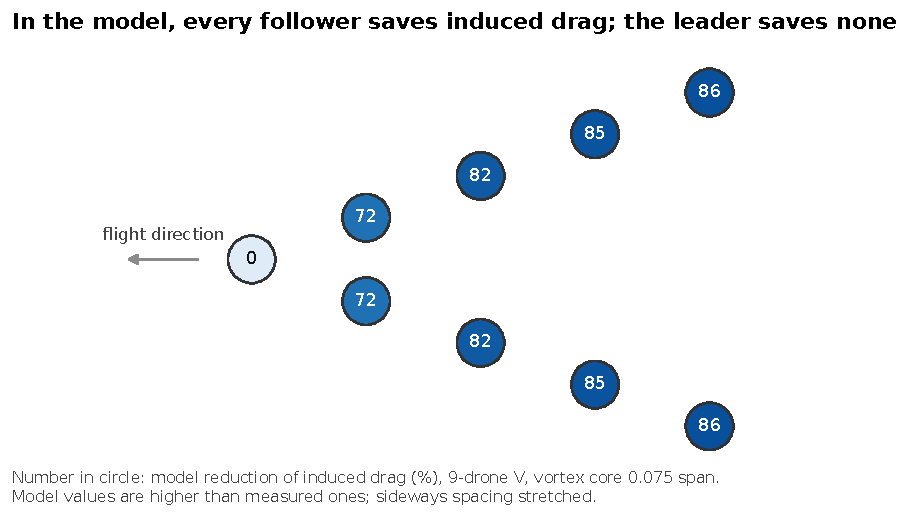
\includegraphics[width=0.7\textwidth]{figures/figA1_formation.pdf}
\caption{In the model, the reduction of induced drag grows with distance behind the leader. Model reduction of induced drag per position in a 9-drone V.}
\label{fig:formation}
\end{figure}

Numerical work finds that every follower in a V or echelon can cut induced drag by about 80\% in the best position \citep{maskew1977}; we adopt this only as model structure.
The model superposes horseshoe vortices with a finite core, a 15\% wing overlap and lateral spacing set by the wing, and it is calibrated against a three-wing vortex-lattice result in which a follower's induced drag falls to about 0.2 of solo \citep{maskew1977}.
The model's reductions are higher than flight tests show (one flight-test condition measured reductions in total drag above 20\% \citep{ray2002}), and the V and echelon layouts give identical fleet means in our setup, which is a consequence of the setup and not a physical finding.
No measured value for the share of induced drag in total power for small drones was found; we sweep it.

\section{Reproducibility}

The numbers in this paper are listed with their source file and field in \texttt{docs/canonical\_numbers.md}; the prediction counts of Appendix~\ref{app:scorecard} are traced row by row in the supplement. All figures except the flow chart of Fig.~\ref{fig:gatechart} are generated by \texttt{scripts/make\_paper\_figs.py} from the result files in \texttt{calib/out/}.
Our search for earlier work, and our checks of the method citations, are recorded in \path{docs/literature/method_citations.md}.
Code, result files and the prediction files (a few passages masked; see \texttt{docs/predictions/README.md}) are at \url{\repourl}.

\end{document}
